
% The subsections written are only suggestions, to display how sections and subsections may look for your thesis



\section{Motivation}

One of the most significant and ancient industries in the world economy, shipbuilding supplies vital services for trade, transportation, and military. Over 50,000 merchant ships trade internationally, transporting a wide range of commodities, according to the International Maritime Organization. Future growth in the global fleet is anticipated as long as there is a growing need for maritime transportation due to population and economic expansion.\\

\noindent However, the ship building industry also faces many challenges and difficulties, such as high costs, long lead times, complex designs, environmental regulations, safety standards, and market fluctuations. Ship life-cycle involves multiple stages, such as design, engineering, fabrication, assembly, outfitting, testing, delivery,operation, retrofitting and maintenance each requiring specialized skills, equipment, and coordination. The ship building production is also affected by various factors, such as weather, human errors, material availability, and quality control. \\


\noindent Thus, creative, safe and effective solutions are required to match consumer demands and expectations while lowering costs and enabling frequent scans, raising the caliber of shipbuilding production. The utilization of robots or operator-based manual data collecting using 360 camera systems in conjunction with lidar and other potential data collection solutions is one of the most promising fields of research and development. Ship design, engineering, fabrication, inspection, 3D reconstruction, safer and efficient marine operations can all be improved by using these technologies, which can make data collection, processing, and analysis quicker, less expensive, and more accurate.\\

\section{Contribution}
\noindent In this thesis, a novel and cheaper method of 3D scanning has been introduced in compare with recent common methods to make 3D models. later this 3D models have been imported to a robotic software for simulation of a virtual robot with different algorithms of path planning and obstacles avoidance for possible fire fighting scenario on the ship or on the terrain. During the thesis process,I found other valuable usage of 3D models in ship industry and construction that talked about it.\\     
\section{Outline}
Figure \ref{fig:Holistic View} shows the structure of the thesis. The thesis consists of five chapters:
introduction, theory, methodology,
results and discussion, and conclusions. \\

\noindent \textbf{Chapter 1} - Motivation, contribution, outline , project description, stakeholders, objective and research questions, general pipeline.\\

\noindent \textbf{Chapter 2} - Literature review and related work provides background
information on the problem and describes related work. \\

\noindent \textbf{Chapter 3} - Methodology contains a description of the developed methodology and materials used during the conducted investigation.\\ 

\noindent \textbf{Chapter 4} - The results and discussion section includes all of the experiments and outcomes of the produced solution, as well as an explanation of the findings.\\

\noindent \textbf{Chapter 5} -Conclusions summarize the main findings and make recommendations for future work.\\

\begin{figure}[H]
  \centering
  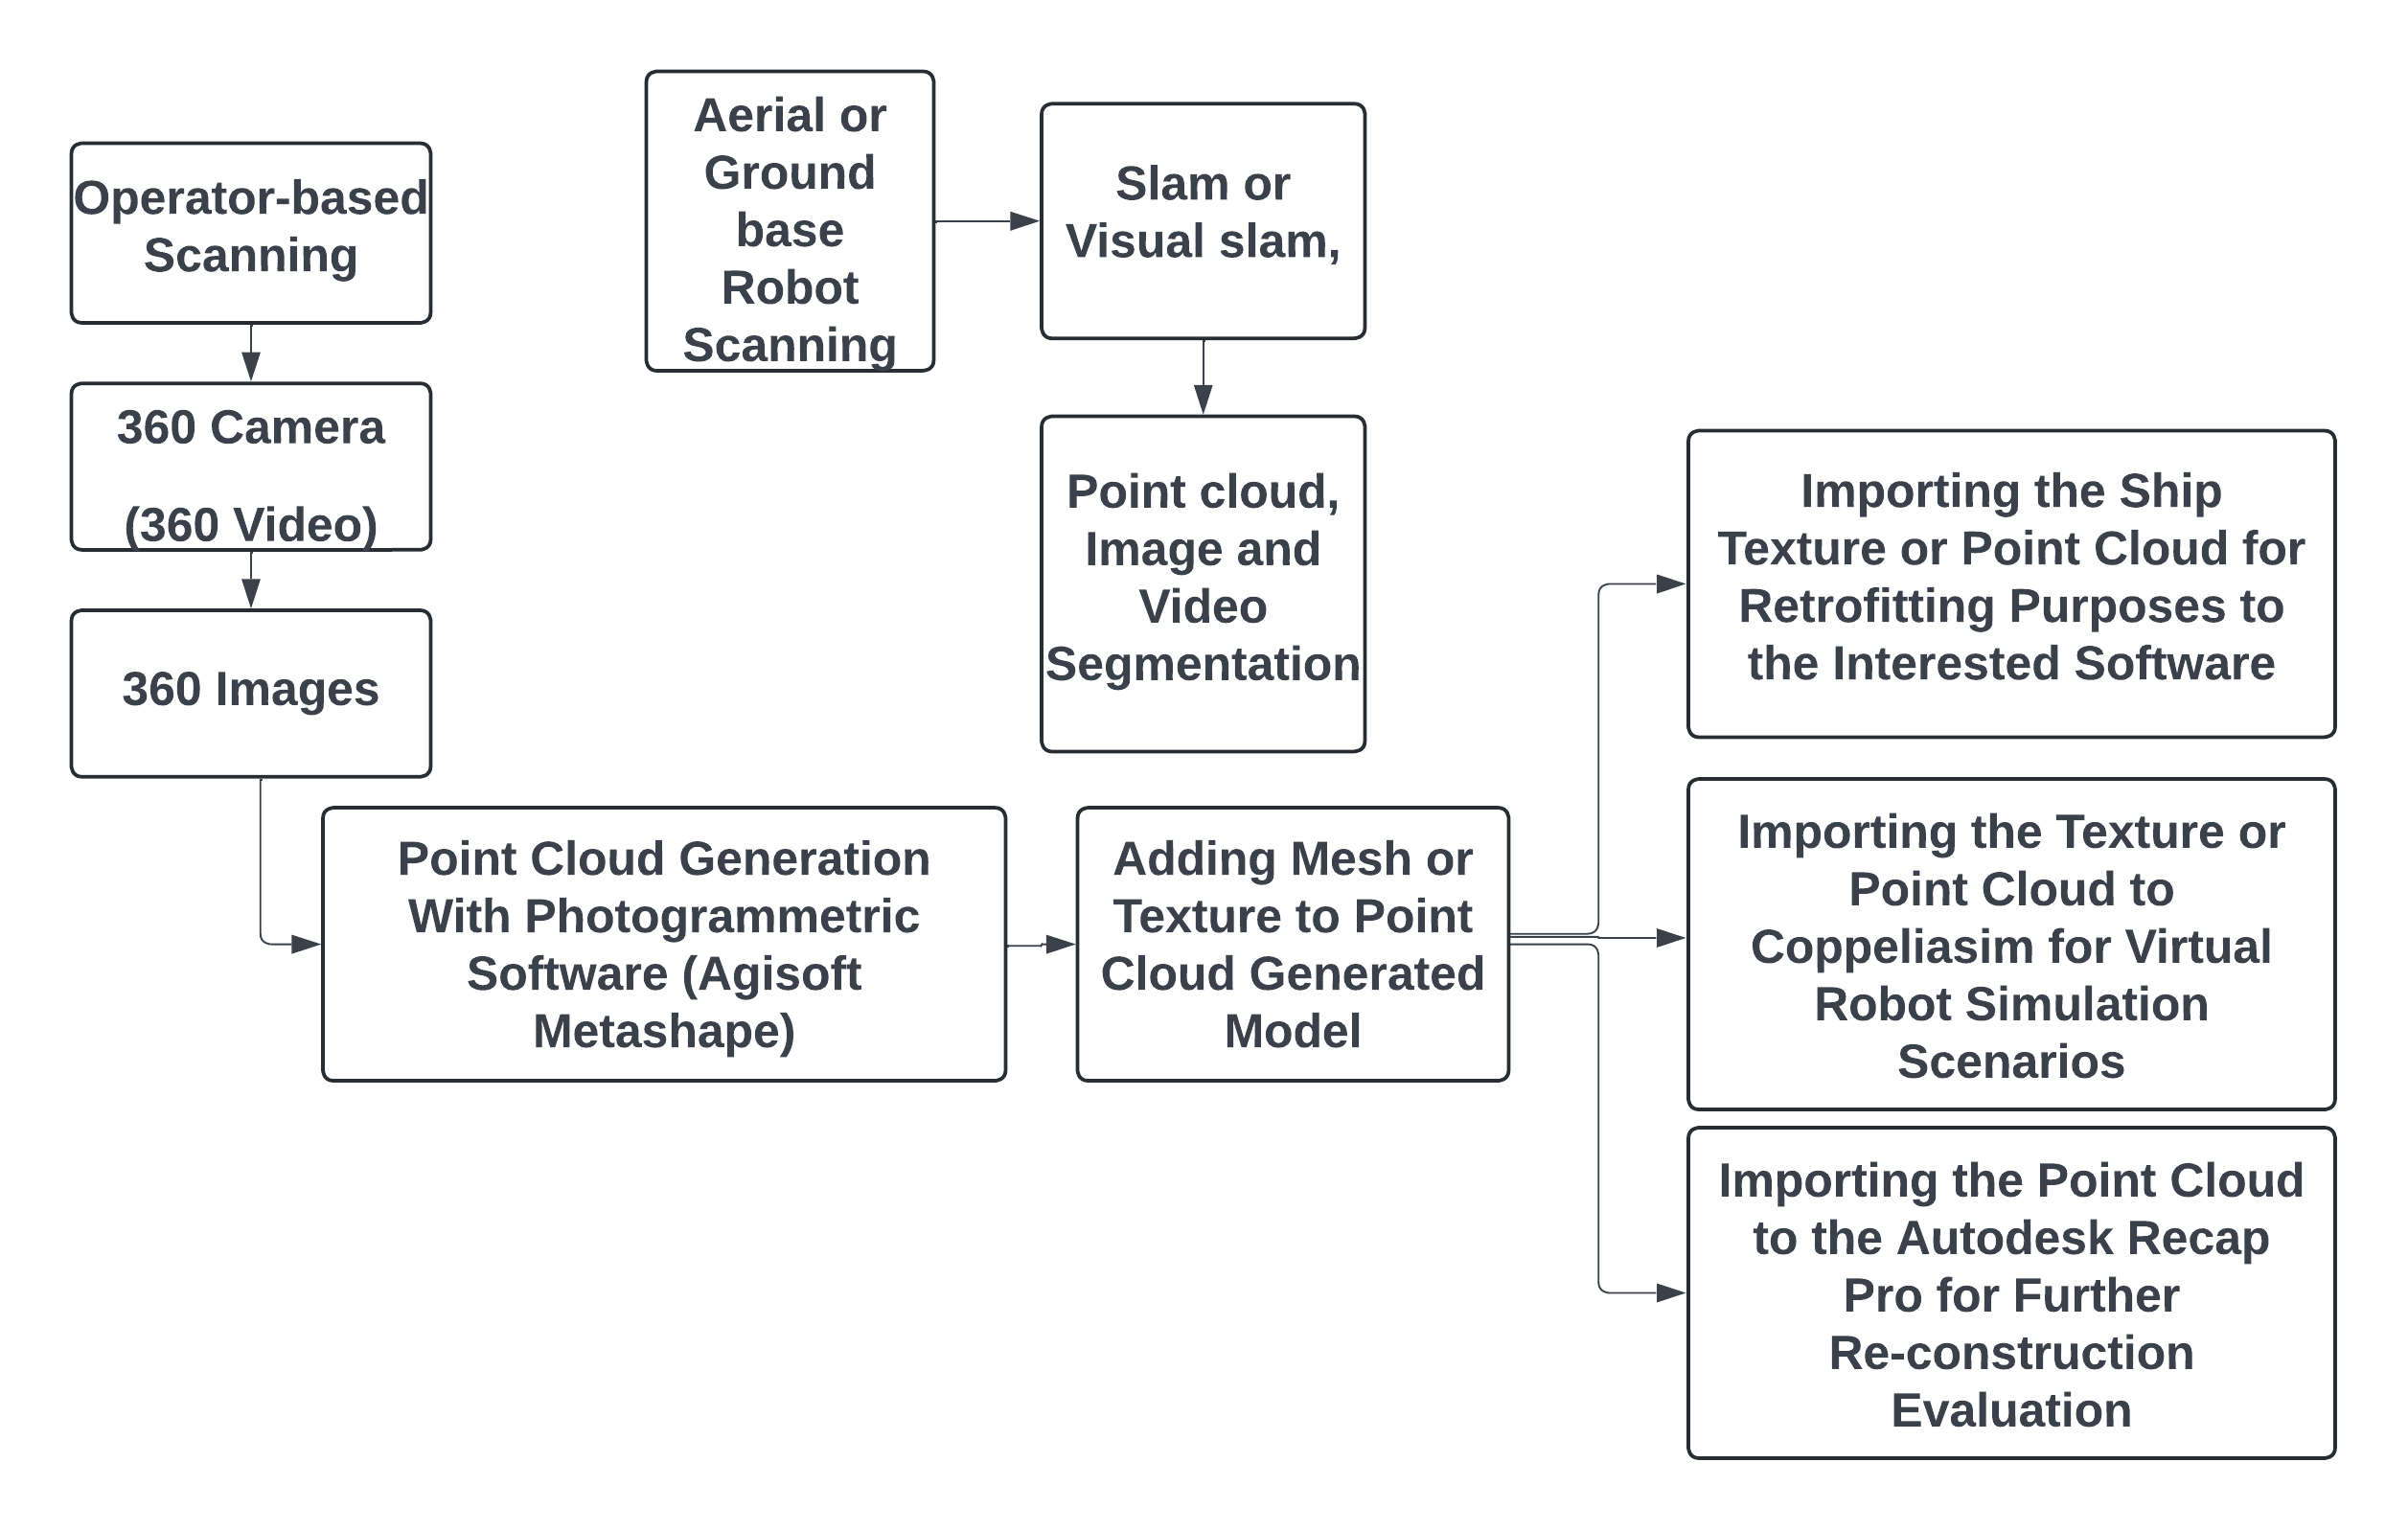
\includegraphics[width= 1.0\textwidth]{Figures/Whole View.png}
  \caption[Holistic View ]{Holistic Flowchart for Human-based and Robot-based Scanning}
  \label{fig:Holistic View}
\end{figure}

\noindent As it is shown in Figure \ref{fig:Holistic View}, two methods planed for this research but just operator-based scanning has been executed in the thesis. And other method concepts (robot-based scanning) mentioned in the literature. Related literature for robot-based scanning (Aerial or Ground) has been explained due to its importance for 3D scanning. 






\section{Project Description}

In this project, I investigate and assess the viability and potential of utilizing operator-based 360$^{\circ}$ scanning technologies for data capturing specifically in the shipbuilding and construction industry then I simulated a robot for fire-fighting scenario in a ship as an outdoor and a hallway as an indoor environment. The work also include some background data on the state-of-the-art scanning techniques and technologies related to shipbuilding industry, and pertinent literature and research on the subjects of neural radiance fields, 360 imaging, photogrammetry, Lidar, and SLAM (for robot-based Scanning).

\subsection{Stakeholders}
A wide range of stakeholders are involved in the discussion of lowering the cost of 3D model re-visioning during ship production and retrofitting in ship life-cycle through innovative technologies. Most of the techniques for 3D scanning and modeling, model-revision during building reconstruction is also applicable. These parties are interested in different aspects of the development, results, and uses of these technologies.\\These are the main parties involved in this situation for ship manufacturing industry. \\

1. Shipbuilding Companies: The main parties who gain directly from lower production costs and increased safety in search and rescue operations and effectiveness in production of the vessels. Technologies that can improve quality, expedite the time to market for new vessels are what they're interested in implementing.\\

2. Ship Owners and Operators: These parties have an interest in how reliable, safe and affordable ships are. Innovations that cut production costs have the potential to minimize vessel acquisition or operating expenses as well.\\

3. Authorities and Safety Organizations:  Organizations that oversee the safety and quality of maritime building. Their area of interest is the impact of emerging technology on adherence to environmental and safety requirements. \\

4. Insurance Companies: companies that offer cargo and ship insurance. They are involved in risk assessment and management since new technologies have the potential to affect the dependability and safety of marine vessels. \\

5. Technology Providers and Innovators: Companies and research institutions that specialize in robotics, LiDAR, photogrammetry, 360 camera systems, and NeRF technologies. They are involved in the research, development, and commercialization of their discoveries.\\

6. Defense Sector: For naval and defense-related shipbuilding, military and defense departments are key stakeholders. They are interested in the strategic advantages and cost savings offered by advanced technologies.\\

\noindent These are the main parties involved for building reconstruction industry.\\

1. Client: Often, the property owner or developer commissions the reconstruction project.\\

2. Structural Engineer: Ensures that the repaired structure is structurally sound and meets safety regulations.\\

3. Contractor:The body responsible for carrying out the reconstruction work in accordance with the project parameters.\\

4. Architect: Plays an important part in designing the reconstruction and ensuring that the new structure fulfills both aesthetic and functional standards.\\

5. Subcontractors: The main contractor hires specialized workers to complete specific jobs such as electrical work, plumbing, and HVAC systems. 

\section{Objective and Research Questions}
Lidar is one of the traditional methods for authentic modelling of buildings for construction purposes. Also use of Lidar in shipbuilding industry for having an accurate 3D model specifically during production and retrofitting is vital. Nowadays with the help of advanced photogrammetry methods, making 3D model is simpler and less expensive than traditional methods. This technology give the equal accessibility to individuals for making 3D models even by a smartphone. After making a 3D model, there are variety of usages for a 3D model, one of them is for simulating a real scenario in a virtual environment like navigating a robot in virtual world that could be at an indoor or inaccessible outdoor location for rescue operations. Another opportunity is adding mesh and texture to the captured point cloud for making a realistic model in retrofitting goals in shipbuilding or construction industry. Due to the lack of industry-applicable resources in operator-based scanning for 3D modeling by 360 degree cameras , I decided to dive into these methods. In this method, an asset scanned and then the video processed with software, and then a point-cloud of that object was made. After visualizing the  point cloud with Agisoft Metashape or other visualizing software it is also possible to make a photo-realistic 3D model of that asset. After adding mesh or even without mesh, 3D model is ready for simulation scenarios, re-construction purposes and ship redesign during production. Mentioned pipeline not only improves the safety and efficiency of marine operations, but it also provides new opportunities for inspection and maintenance chores that were previously difficult owing to the hostile marine environment.  \\

\noindent In this research, we try to address the following questions:\\

\noindent $RQ_1-$ What are the benefits of scanning an object with 360 -degree camera?  \\

\noindent In scanning process I used 360 camera and a software to separate the scanned frames and then stitch the frames or photos together to make a model or point cloud. (Complete answer is in conclusion chapter)



\noindent $RQ_2-$ What are the advantages of using captured point cloud for 3D reconstruction purposes with application in construction industry\\

\noindent After scanning the building, it is possible to import the point cloud to a software and start redesign.(Complete answer is in conclusion chapter)\\

\noindent $RQ_3-$  How to benefit from captured point cloud for more efficient ship maintenance? (This question addressed in literature review)\\
\noindent After scanning of the intended rooms or components in the ship for making a dense point cloud, we can import point cloud on the original CAD model for re-design.(Complete answer is in conclusion chapter) \\ 


\noindent $RQ_4-$ How to investigate the simulation of a robot in a 3D virtual world for safer marine operations?\\
We need a high fidelity virtual environment with real-world physics for this rescue robot to have an interactive and realistic training scenarios. This environment could be a point cloud or a textured model. After importing this model to Coppeliasim robotic simulation software, I fine tuned the robust algorithm parameters for getting optimized result.(Complete answer is in conclusion chapter)    





